The single machine implementation uses a thread-safe map internally to manage topics and subscribers. Each subscriber is put into its own thread\footnote{Service is implemented in Go\citep{golang}, where a thread is a go-routine.}. Every time a message is published, broker will first deliver the message to the subscriber threads of the message topic, and thereafter the message will be transported to clients in each thread, as shown in Figure 2. 

\begin{figure}[H]
	\centering
	\begin{tikzpicture}[shorten >=1pt,node distance=2cm,on grid,auto]
		\node[state] (0) {msg 1};
		\node[state] (1) [right=of 0]{msg 2};
		\node[state] (2) [node distance=2.5cm,below=of 0]{topic 1};
		\node[state] (3) [node distance=2.5cm,below=of 1]{topic 2};
		\node[state] (4) [node distance=2.5cm,below left=of 2]{sub 1};
		\node[state] (5) [node distance=2.8cm,right=of 4]{sub 2};
		\node[state] (6) [node distance=2.5cm,below right=of 3]{sub 3};
		\path[->]
			(0) edge node {} (2)
			(1) edge node {} (3)
			(2) edge node {} (4)
			(2) edge node {} (5)
			(3) edge node {} (5)
			(3) edge node {} (6);
	\end{tikzpicture}
	\caption{Single Machine Model}
\end{figure}

\begin{figure}[H]
	\centering
	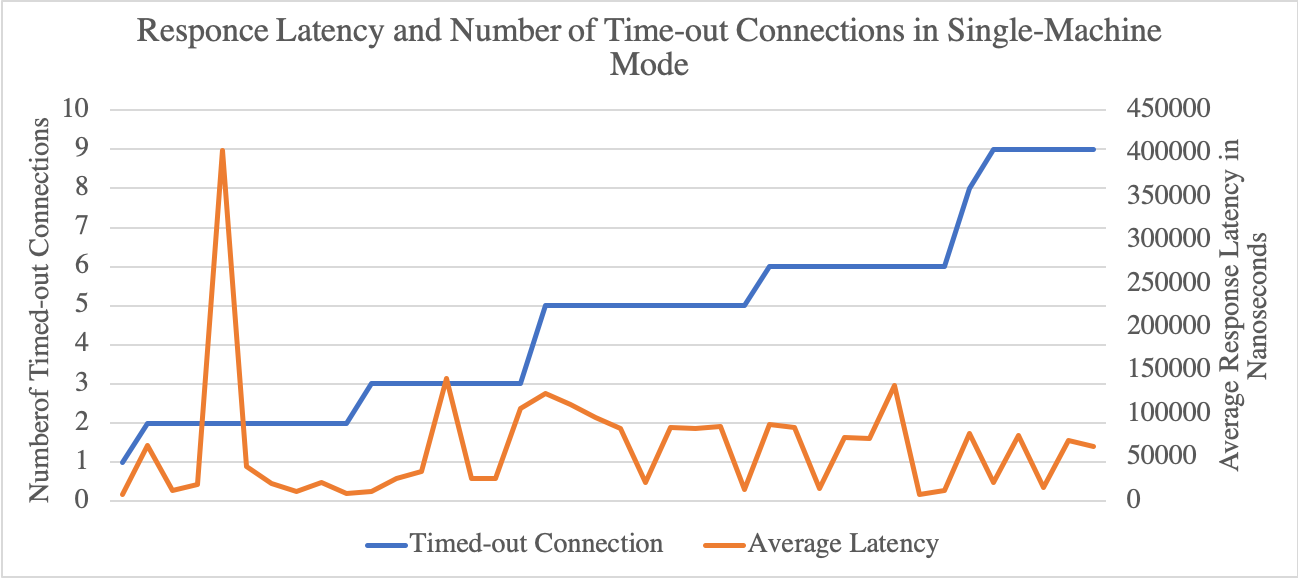
\includegraphics[scale=0.33]{figure/single-machine/performance.png}
	\caption{Single-Machine Performance}
\end{figure}

Figure 3 demonstrates the performance of a single-machine service throughout load-testing. In average a single-machine service could finish a round of messages within 50 milliseconds. Several clients were blocked in the process and timed out; one possible reason could be that there is only one simulation process, so the client threads were locked, or maybe neglected, during user context switching. The issue should be negligible since the overall time-out rate is less than 0.5\%. The researchers later applied load-testing using the same setup to find out the maximum capacity of this implementation, and statistics showed that such a service could be handle 20000 clients with roughly 3\% timeout rate.
